\documentclass{jarticle}
\usepackage{robomech}
\usepackage[dvipdfmx]{graphicx}

\begin{document}
\makeatletter
\title{筋骨格ヒューマノイドにおける面状牽引構造を有する関節の開発}
{}
{Development of Joint with Planar Traction Structure on Musculoskeletal Humanoids}
{}

\author{
\begin{tabular}{lllll}
 \quad \hspace{5zw}○\hspace{1zw}鬼塚 盛宇 & (東大)&\hspace{3zw}& 学\hspace{1zw}河原塚 健人 & (東大)\\
 \quad \hspace{5zw}学\hspace{1zw}牧野 将吾 & (東大)&\hspace{3zw}& 学\hspace{1zw}新城 光樹 & (東大)\\
 \quad \hspace{5zw}学\hspace{1zw}都築 敬 & (東大)&\hspace{3zw}& \quad\hspace{1zw}中島 慎介& (東大)\\
 \quad \hspace{5zw}正\hspace{1zw}浅野 悠紀 & (東大)&\hspace{3zw}&\quad \hspace{1zw}岡田 慧 &(東大)\\
 \quad \hspace{5zw}\quad\hspace{1zw}川崎 宏治 & (トヨタ自動車)&\hspace{3zw}& 正\hspace{1zw}稲葉 雅幸 & (東大)\\
 &\\
 \multicolumn{5}{l}{\small Moritaka ONITSUKA, The University of Tokyo, onitsuka@jsk.imi.i.u-tokyo.ac.jp}\\
 \multicolumn{5}{l}{\small Kento KAWAHARAZUKA, Shogo MAKINO, Koki SHINJO, Kei TSUDZUKI}\\
 \multicolumn{5}{l}{\small Yuki ASANO, Kei OKADA, Masayuki INABA, The University of Tokyo}\\
 \multicolumn{5}{l}{\small Koji KAWASAKI, TOYOTA MOTOR CORPORATION}
\end{tabular}
}
\makeatother

\abstract{
\small
In the musculoskeletal humanoid trying to make use of advantage of the human body by mimicking the its structure, ligaments that constrain the joint movement softly and form complex range of motion are no less important skeletal traction structure than muscles which actuate skeleton. However, the conventional linear traction structure with wire can not maintain stable tension depending on the posture change of the joint. In this study, we propose planar traction structre as skeletal traction structure, and describe and evaluated its advantages. Also we attach the planar collateral ligaments to the knee joint, and reaize screw-home movement like human knee joint.
}

\date{} % 日付を出力しない
\keywords{Biomimetic Humanoid, Ligaments, Planar structure}

\maketitle
\thispagestyle{empty}
\pagestyle{empty}

\small
\section{はじめに}
筋骨格ヒューマノイド\cite{SR2017:asano:design}は人体を模した身体構造を特徴とし、骨格の周囲にアクチュエータとして筋を配置して駆動する人型ロボットである。人体模倣を規範として設計され、人の様な巧みな身体動作が期待される。人体の骨格に見られる柔軟な劣駆動多節構造を有する背骨や特異点の存在しない開放型球関節が実現されていることに加え、冗長に多数取り付けられた筋によって関節の可変剛性制御を可能としている。人のような動作の実現のためには、人の関節の構造や機能に学ぶ必要があり、重要な役割を持つ構造の一つとして靭帯が挙げられる。

靭帯は筋と同様に関節をまたいで骨格同士を牽引するが、関節に対し受動的に働くという点で役割が異なる。靭帯の主な機能は関節に拘束を設け骨格間の相対運動の方向や可動域を決定することである。筋が脱力していたり有効に張力が伝えられない場合も受動的な力を関節に及ぼし、脱臼を防ぐなど関節の安定化に貢献している。多くのロボットでは軸受けや関節リミット機能をリジッドなハードウェアで実装しているが、リジッドな関節拘束は衝撃をハードウェアで吸収できず致命的な破壊が起きうる。人のような動作に耐え、柔らかで複雑な可動域を持つ関節を実現するためには靭帯を含めた関節構造を考える必要がある。

柔らかい素材による関節の拘束についての研究として開放型球関節の並進運動を拘束する間接包\cite{Biorob2018:fujii:capsule}や膝関節の運動を転がり曲面に拘束する靭帯\cite{RoboSym:sonoda:ligaments}ついての研究、人の手を精巧に模したロボットハンドで編地とゴムによって靭帯を実装した研究\cite{ICRA2016:xu:hand}がある。\cite{Biorob2018:fujii:capsule}は関節全体をゴムで包むことで人と同様の可動域を実現しつつ脱臼を防いでいるが、ゴムの強度と可動域にトレードオフがあり、広い可動域を確保するために強度を犠牲にしている上、ゴムの劣化も生じる。\cite{RoboSym:sonoda:ligaments}ではいくつかの繊維を束ねた靭帯によって人の膝における転がり運動への拘束を実現しているが2次元運動のみを扱っており、膝の回旋は考慮に入れていない。\cite{ICRA2016:xu:hand}では人体の関節構造を実装する際に靭帯を設けることで物体の柔軟な把持を可能とし、人体の手の構造における靭帯の有効性を示している。

人体に見られるような曲面形状を持った関節を柔らかに拘束するためには、引っ張り方向に強いワイヤや布等を用いた靭帯が適切だと考えられるが、3次元的に様々な方向への回転を許す場合、ワイヤによる骨格間の牽引は曲面上でワイヤがずれて骨格の支持ができない、機構の突起や隙間に引っかかりやすいなど実装上の問題が発生する。これは筋にも生じる問題であり、骨格に機構や組織をまとわせる筋骨格系に特有の問題である。\cite{Humanoids2011:osada:planar}では面状筋を実装することでこの問題を解決している。そこで靭帯についても人体に見られる骨格と面で接触するような構造を積極的に取り入れることでこれらの問題の解決に取り組む。

本研究では骨格同士を牽引する構造として靭帯に着目し、人体における面状組織を模した構造、面状牽引構造を有する靭帯を球体関節に実装し、面状牽引構造の評価と人体の関節と同様の機能を実現する。
まず面状牽引構造の利点について述べ、ワイヤを非線形弾性要素とみなしてモデル化して評価を行う。次に実際に球体関節周りにワイヤで作った靭帯を取り付けて外力をかけ、モデルと同様の結果が得られることを確認する。最後に膝関節の側副靭帯を布で実装し人と同様の機能が実現されていることを確認する。

\section{面状牽引構造}
\subsection{面状牽引構造の利点}
筋や靭帯などの骨格間牽引構造について、ワイヤや紡錘形のように骨格に点で取り付けられ線状に接触するものを線状牽引構造とし、骨格に線で取り付けられ面で接触する構造を面状牽引構造とする。\reffig{fig:schema}に線状牽引構造と面状牽引構造の比較の模式図を示す。面状牽引構造は次の利点を持つ。

\begin{figure}[tb]
 \centering
  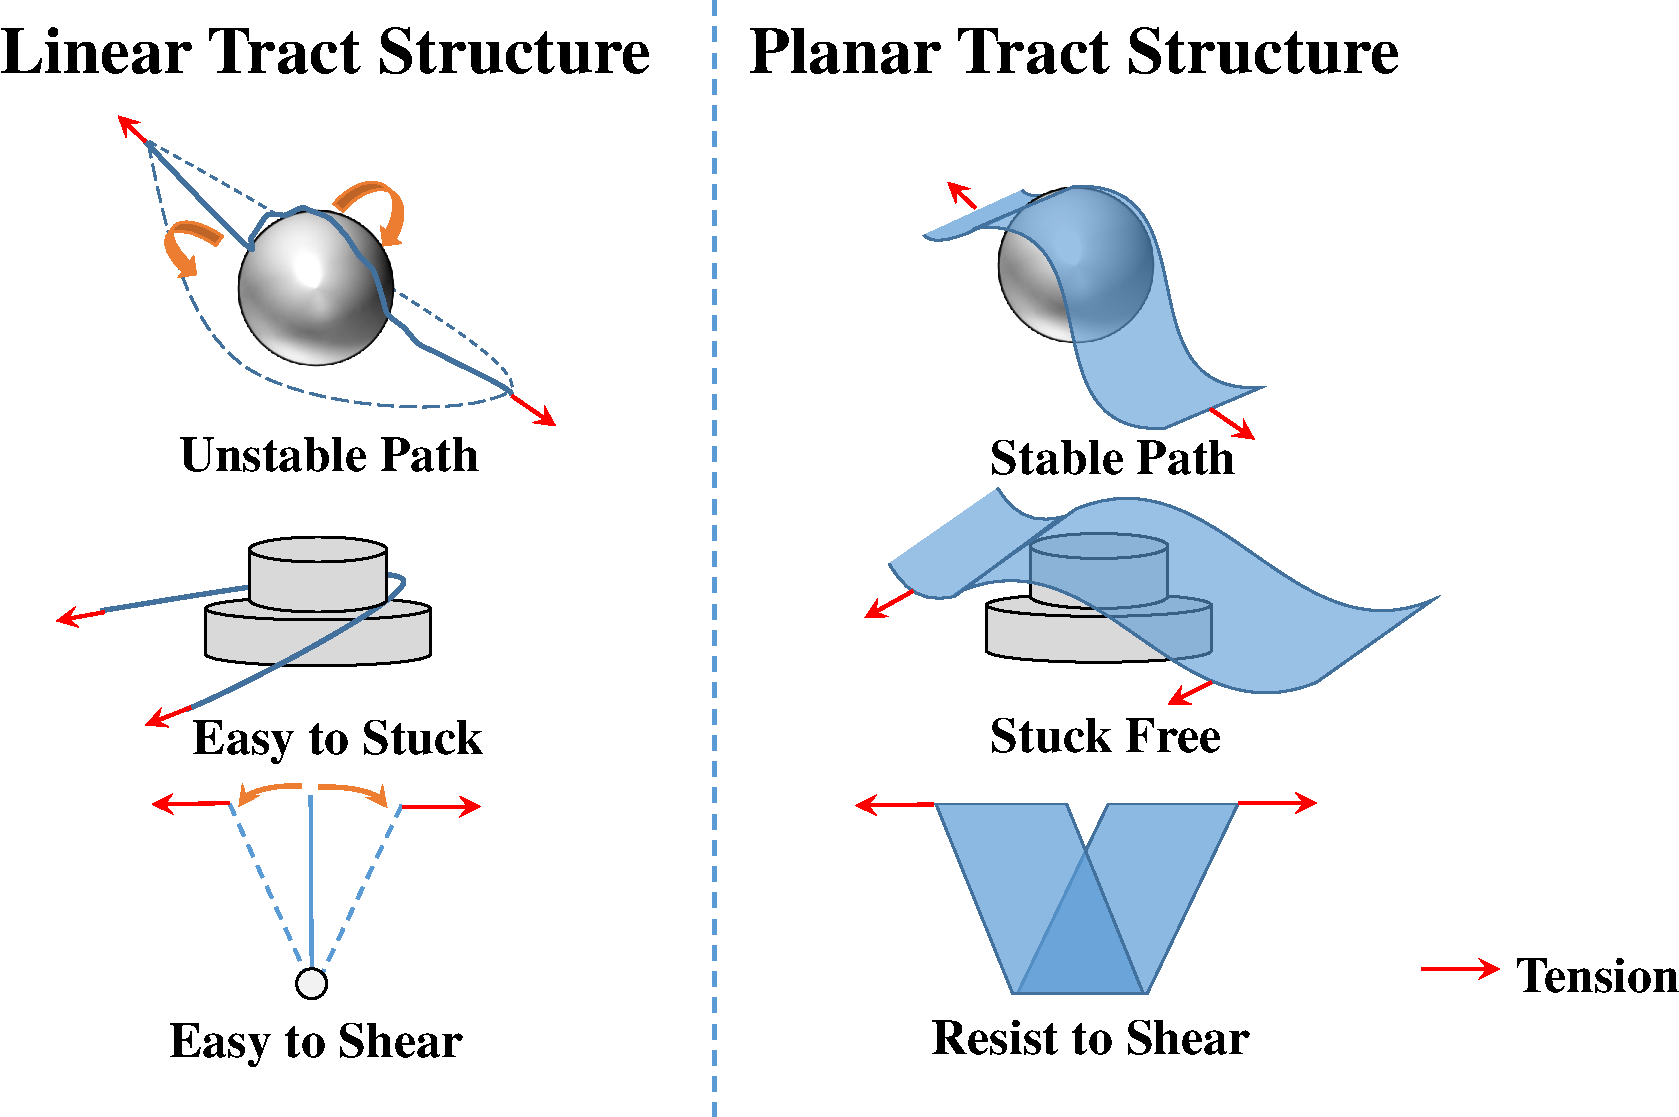
\includegraphics[width=1.0\columnwidth]{figs/schematic-comparison-of-structure.pdf}
  \vspace*{-4mm}
  \caption{Comparison between linear traction structure and planar traction structure.}
  \label{fig:schema}
\end{figure}

\begin{enumerate}
\item 面構造による骨格曲面との安定的接触

  球体関節などの曲面形状を持った骨格に牽引構造が接する時、牽引構造の両側には張力がかかっている場合力学的なポテンシャルが低い経路を取るように形状に変形していく。面状牽引構造の場合、面が骨格曲面に応じて変形し骨格が面の内側から外側に逸脱することは無いが、線状牽引構造の場合容易に逸脱する。例えば球面に対してワイヤをかけると球面の子午線は不安定な領域なのでワイヤがちょうどかかることはほぼありえない。靭帯や筋の場合、関節が牽引構造の外側に出てしまい、関節の支持や制御が不可能になる\cite{Humanoids2011:osada:planar}。面状牽引構造は線状牽引構造に対して骨格と安定した接触を保つことで、骨格姿勢が変化して関節と接触する向きが変わっても、安定してその張力を関節に伝えることができる。

\item 面構造による機構への引っ掛かり防止

  線状牽引構造は骨格との接触面積が小さく、機構上生じてしまう溝や角に引っかかりやすい。これによって意図しない張力が生じ、例えばワイヤの断裂や関節トルク不足が生じていた上、容易に機構に引っかかるので動作の際に試行によって機構への引っかかり方が変わってしまうなどの問題が生じていた。
  %% \cite{ROBOMECH2016:katayama:cover}では筋に外装を取り付けワイヤと骨格との摩擦を抑えることでワイヤの断裂を防いでいる。
  面状牽引構造は張力がかかっている場合骨格形状を覆うように変形するため、溝や角に引っかかりにくい。

\item 弾性の異方性の緩和

  端点が位置のみ拘束を受け、回転について自由度を持つとすると、線状牽引構造は引っ張り方向(\reffig{fig:comparison}の${y}$方向)にはその弾性によって力を受けることができるが、せん断方向(\reffig{fig:comparison}の${x}$方向)は力を受けづらい。一方面状牽引構造は繊維同士が干渉しあうことで線状牽引構造に比べてせん断方向の力も受けることができると考えられる。

\end{enumerate}

一方欠点としては、面状牽引構造を筋に適用する場合、モータによって巻き取れないので筋のストロークがワイヤに比べて短く、ワイヤのように容易に折り返せないので、ワイヤによる線状牽引構造よりも筋経路の汎用性に欠けるという点が挙げられる。Osadaらの研究\cite{Humanoids2011:osada:planar}では筋を多重に折り返して面状牽引構造を実装することで設計自由度の高さを実現しているが、プーリとワイヤとの摩擦が蓄積されていくことでワイヤの張力が面全体に伝達されず、ワイヤが平行に走っているので上述の3の利点で述べた弾性の異方性は残ったままである。また面状牽引構造は骨格と面で接触するので摩擦の面で不利だと言える。

面状牽引構造においてワイヤを平行に取り付けただけの構造は好ましくない。このことも含め、次に面状牽引構造の弾性をワイヤの集まりとしてモデル化し、線状牽引構造の複数の牽引方法と比較して評価する。

\subsection{面状牽引構造の弾性の評価}\label{sec:hoge}
\reffig{fig:comparison}に線状牽引構造と面状牽引構造の比較の模式図を示す。布の形状のモデル化としてはエネルギー最小化に基づいてBreen\cite{Breen:1994}らによって正確なモデルが得られているが、本研究では面上の二方向の外力に対する弾性のみを考えるため、布のモデルとして\reffig{fig:comparison}のParallel-Crossにあるとおり、並行なワイヤと交差するワイヤによって牽引されるトラス構造で簡略化して考える。また線状牽引構造との比較として並行なワイヤのみで牽引した場合(\reffig{fig:comparison}Parallel)と交差したワイヤのみで牽引した場合(\reffig{fig:comparison}Cross)を考える。ワイヤの張力と伸びの間に次の関係が成り立っているとする。
\begin{equation}
  T = \exp(K\max(0,(l-l_0) - l_d))
\end{equation}
${T}$は張力、${K}$はワイヤの剛性を示し現在のワイヤの長さ${l}$と自然長${l_0}$の差分にかかる。ワイヤの伸びについて$(-\infty,l_d]$の範囲に不感帯を設け、一定以上の伸びに対して非線形かつ急激に張力を増大させるワイヤを仮定して指数関数として表す。左辺は単位を持たない値になるが、異なる牽引構造の間の相対的な
違いを見るため、張力${T}$のスケールを表す定数は1Nとして考える。
${K=1.0}$、${K=0.5}$mmとし、${l_0}$は取り付け位置の間隔が\reffig{fig:comparison}でいうところの${x}$方向に200mm、${x}$方向に20mm離れているとして\reffig{fig:comparison}の各構造についてワイヤの張力と端点の変位の関係を計算した。ワイヤの本数をそれぞれ四本とし、その結果を\reffig{fig:simulation}に示す。

\begin{figure}[tb]
 \centering
  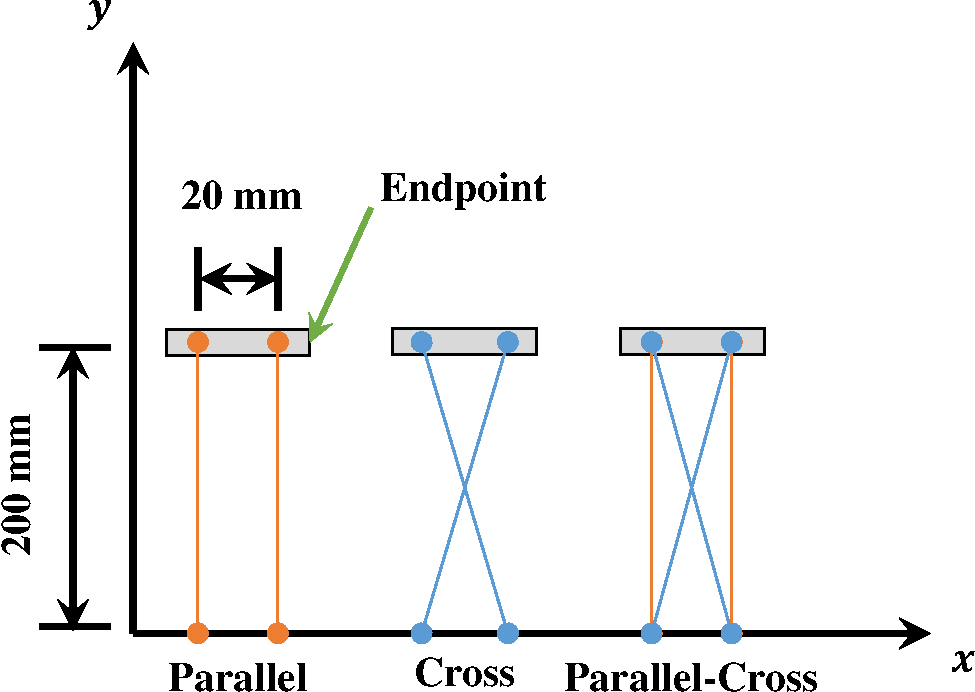
\includegraphics[width=0.7\columnwidth]{figs/schematic-comparison-of-ligaments.pdf}
  \vspace*{-4mm}
  \caption{Schematic diagram of traction structures. Planar structure is simplified as wires what pulls parallel and cross direction}
  \label{fig:comparison}
\end{figure}

\begin{figure}[tb]
 \centering
  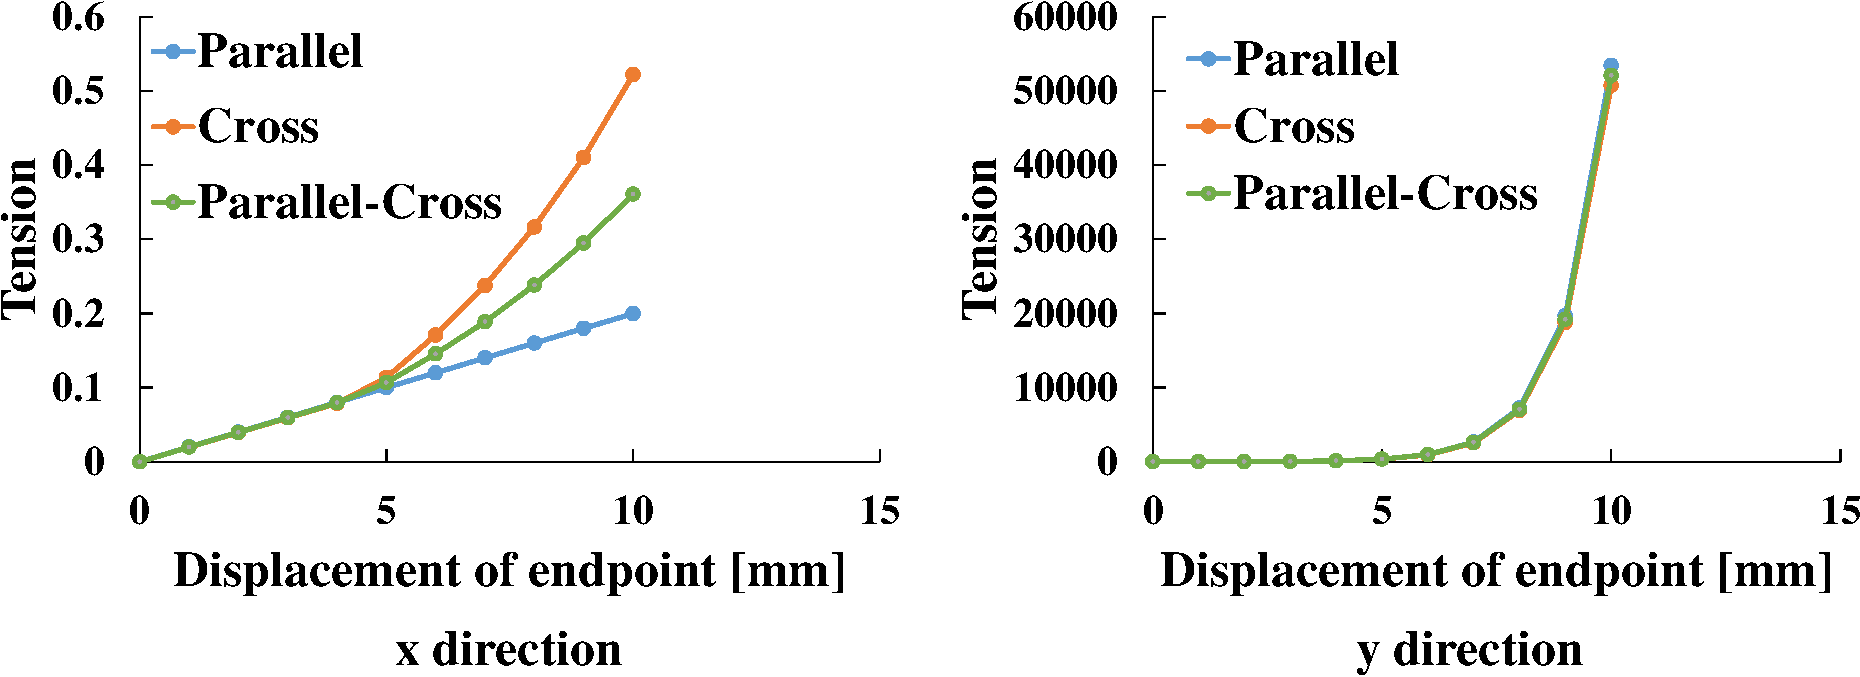
\includegraphics[width=1.15\columnwidth]{figs/xy.pdf}
  \vspace*{-4mm}
  \caption{Simulation result of relation wire tension and the endpoint displacement. the endpoint is moved to x and y direction respectively.}
  \label{fig:simulation}
\end{figure}
%% \begin{figure}[tb]
%%  \centering
%%   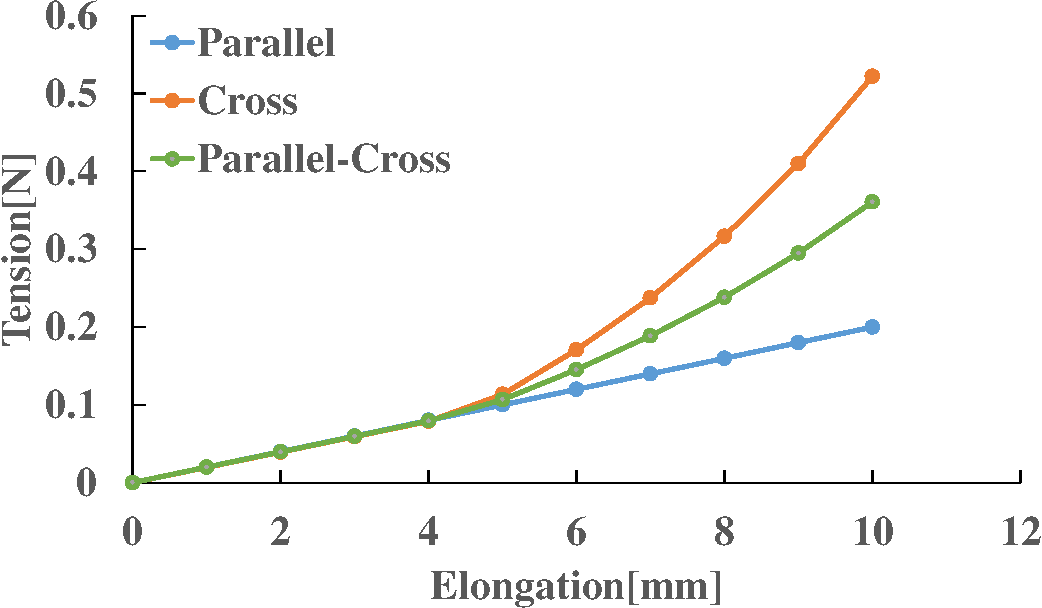
\includegraphics[width=1.0\columnwidth]{figs/x.pdf}
%%   \vspace*{-4mm}
%%   \caption{Simulation result of wire tension. Endpoint of traction structures moves to x direction.}
%%   \label{fig:simulation-x}
%% \end{figure}
%% \begin{figure}[tb]
%%  \centering
%%   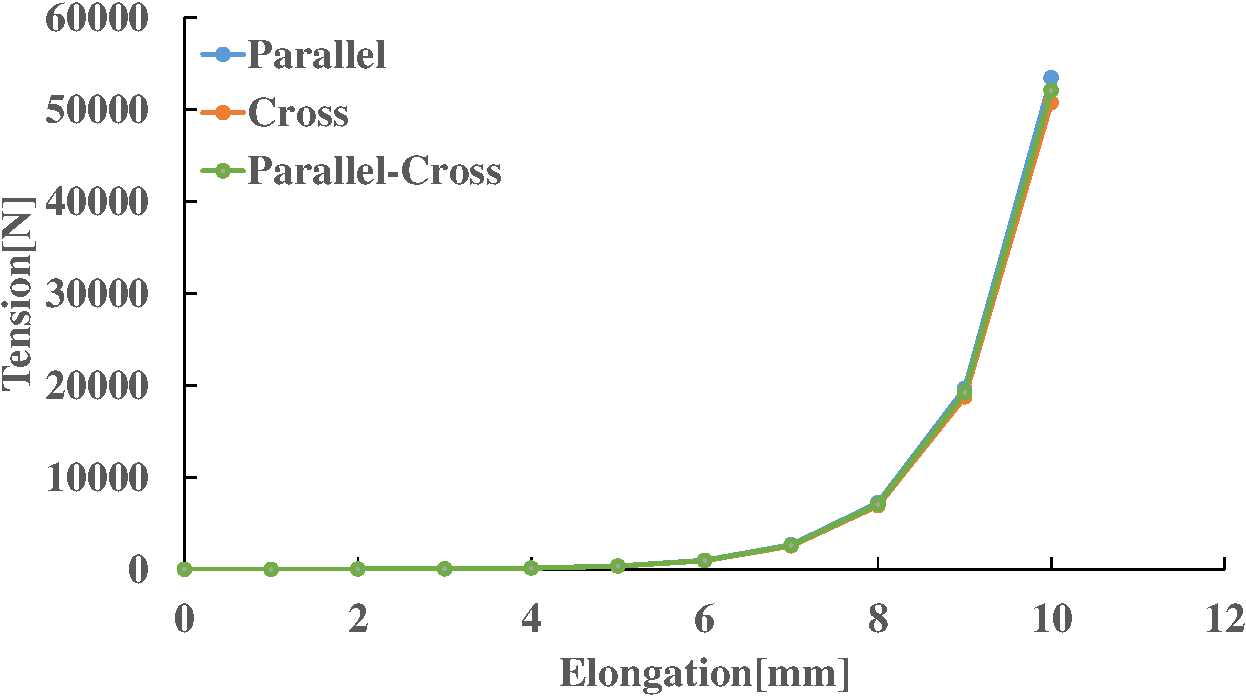
\includegraphics[width=1.0\columnwidth]{figs/y.pdf}
%%   \vspace*{-4mm}
%%   \caption{Simulation result of wire tension. Endpoint of traction structures moves to y direction.}
%%   \label{fig:simulation-y}
%% \end{figure}
傾向として平行構造よりも交差構造の方が${x}$方向、すなわちせん断方向の力を受けることができることがわかる。一方引張方向(${y}$方向)については平行構造が最も張力を発揮しているものの、10mmの伸びに対していずれも約54000[N]まで発揮しており大きな差は見られなかった。両方向について面構造(Parallel-Cross構造)は両構造の中間の性能を持っており、ここから並行と交差の両構造を有する面状牽引構造は線状牽引構造の弾性の異方性をある程度緩和していると考えることができる。ワイヤの交差による骨格の牽引も有効であることが示されたが、前節で述べたとおり骨格との接触を考慮すると面状牽引構造に優位性がある。

\section{面状側副靭帯による関節受動トルク}
本章では前章で述べた面状牽引構造の有効性を実機で示すため、球体関節周りに側副靭帯を取り付けその機能を検証する。まず2.2節で述べた面状牽引構造の弾性を実機で評価し、続いて人体の膝関節に見られる終末強制回旋機能が側副靭帯による受動トルクで実現されることを確認する。

\subsection{球体関節周りの靭帯による関節剛性の比較}
2.2節で示した結果を実際に検証するため、各牽引方法を実際にワイヤを使って球体関節周りに実装した。球関節は河原塚らによって開発された擬似球関節\cite{ROBOMECH2018:kawaharaduka:joint}を用いる。人体の関節に見られる球面の中に複数のセンサと回路が収納され、一点で交わる三本の回転軸を持っている。
ワイヤはDyneemaを使用した。また材質や断面積が異なるので単純な剛性の比較はできないが、東レの鎧布を用いた面状牽引構造についても同様に実装した。関節に靭帯を実装した装置の概観を\reffig{fig:testbed}に示す。

\begin{figure}[tb]
 \centering
  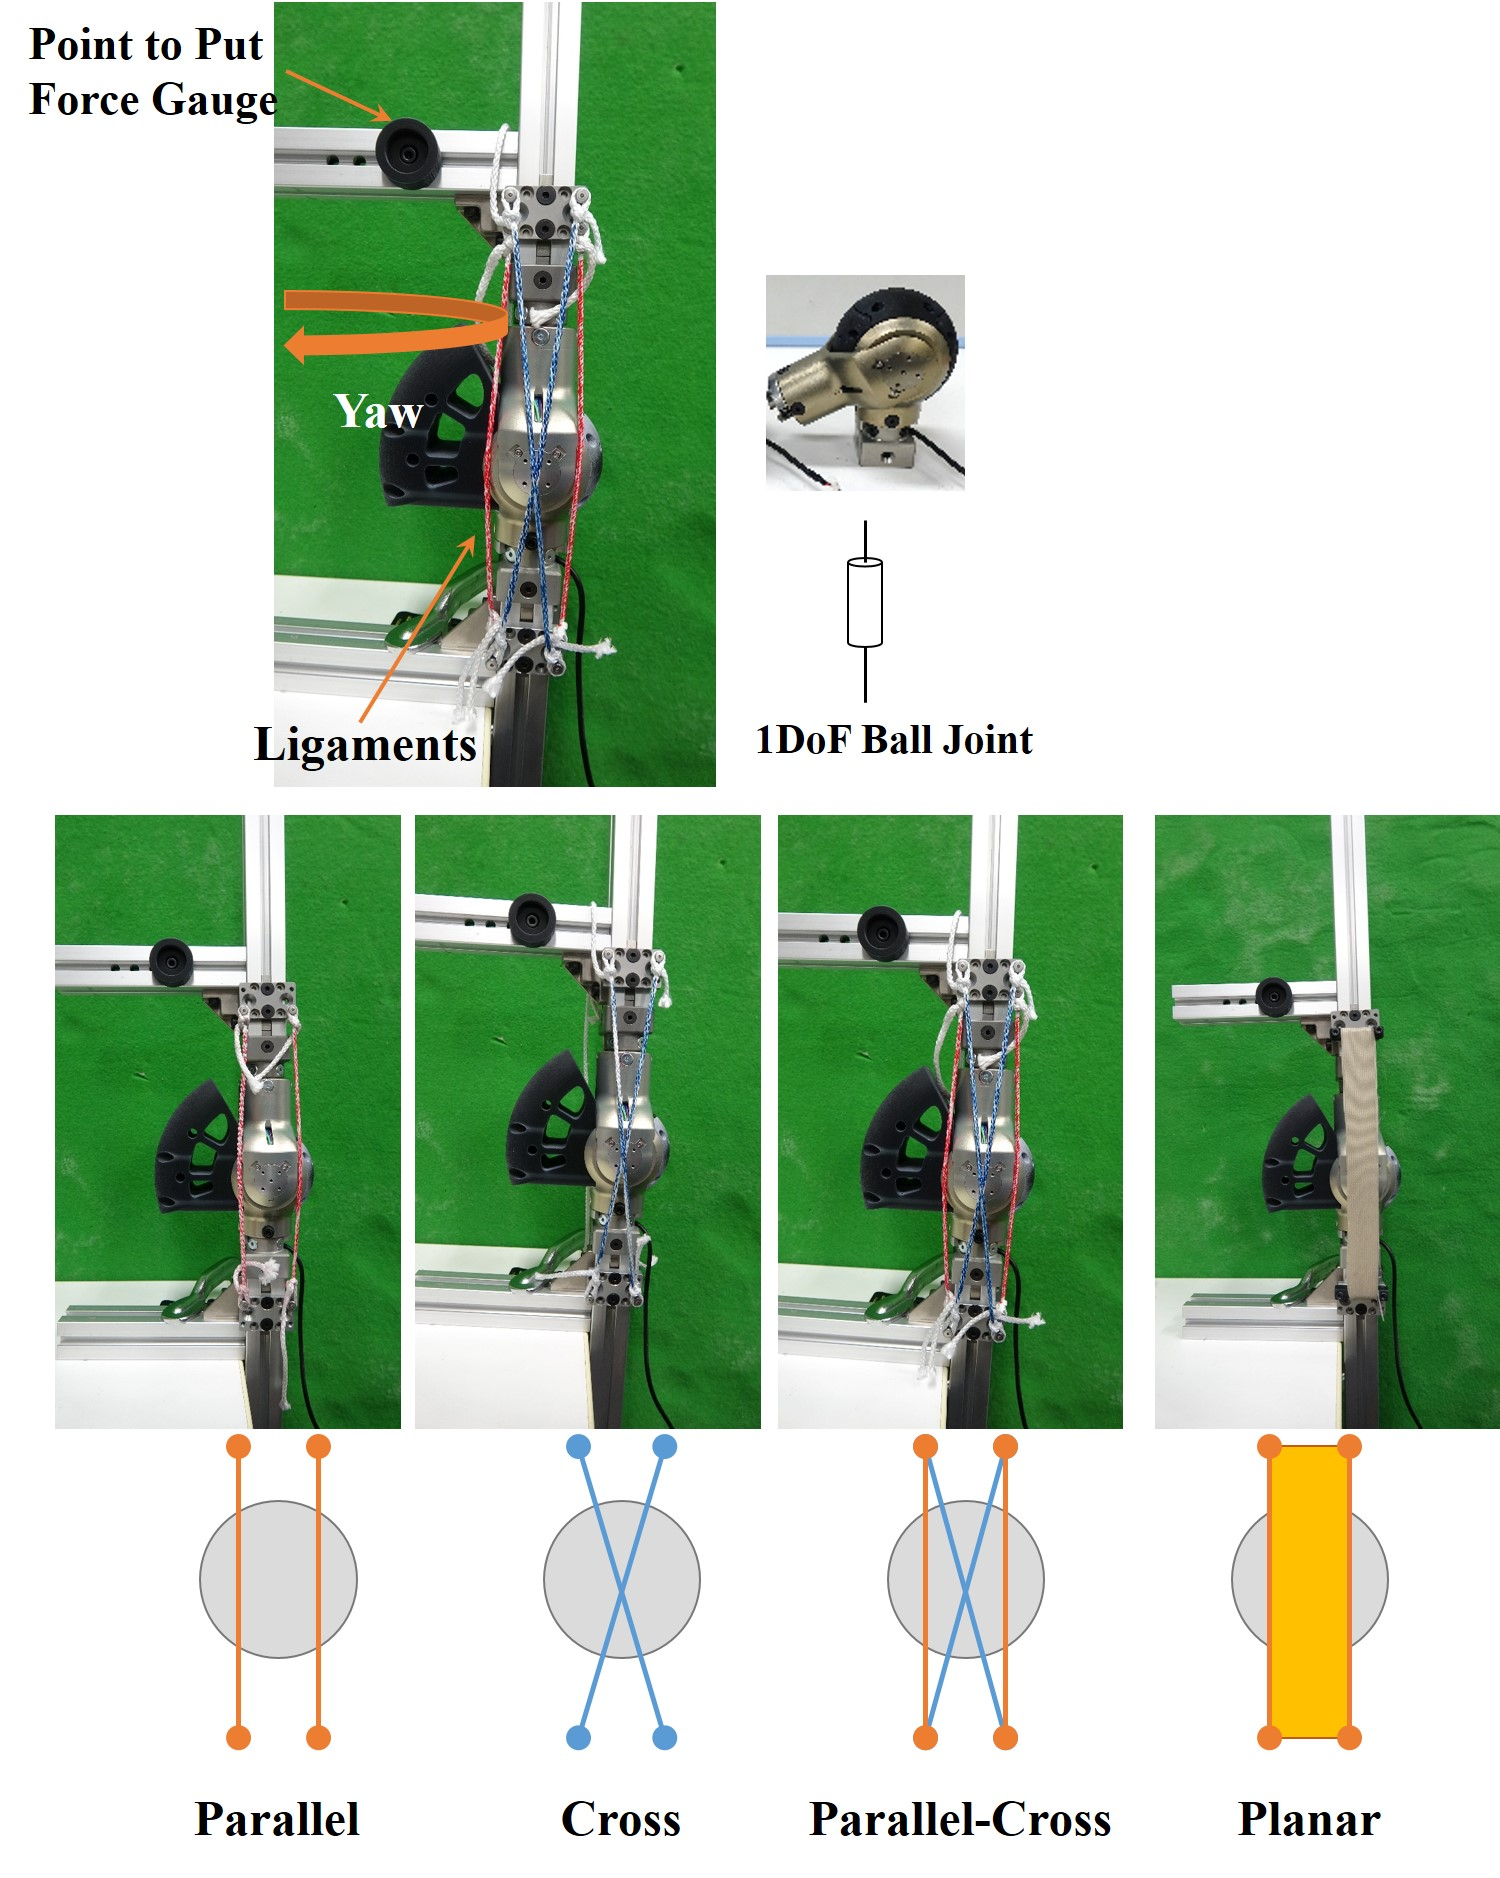
\includegraphics[width=1.0\columnwidth]{figs/experimental-setting.jpg}
  \vspace*{-4mm}
  \caption{Experimental settings for passive compliance by collateral ligaments.}
  \label{fig:testbed}
\end{figure}

牽引方法に応じて大きな差異が見られたせん断方向について調べるため、擬似球関節の二本の回転軸を固定し、回旋方向(\reffig{fig:testbed}のYaw方向)方向のみ回転を許した状態で、軸から60mmの位置にフォースゲージを介して7Nまで力をかけることで、ワイヤと布の各牽引方法について回旋トルクと関節の回旋方向の移動角の関係を検証する。その結果を\reffig{fig:passive-compliance}に示す。

ワイヤの3種類の牽引方法について、Prallel、Prallel-Cross、Crossの順に回旋に対し強い復元トルクを発揮するという\reffig{fig:simulation}と同様の結果が得られた。布についても同様の傾向の復元力が見られている。また布による靭帯はワイヤによる靭帯で生じていた骨格への引っ掛かりが生じなかった。これにより柔らかな面状の素材を用いた関節拘束が実現できたが、ワイヤと布の両者について0.5Nm未満のトルクで10deg以上回旋し、十分な関節剛性が得られなかった。受動的に張力を発揮して関節を保持するためには、骨格に靭帯をとりつける際に張力を保った状態で取り付けることが必要になる。ワイヤを捻ることによって張力を維持して固定しており、面状牽引構造のための布についても取り付け部品に巻きつけて固定することで張力を維持した状態で取り付けたが、十分な張力を出すことが出来なかった。関節の動きを阻害しない骨格へのコンパクトな取り付けと十分な張力維持の両立は今後の課題となる。

\begin{figure}[tb]
 \centering
 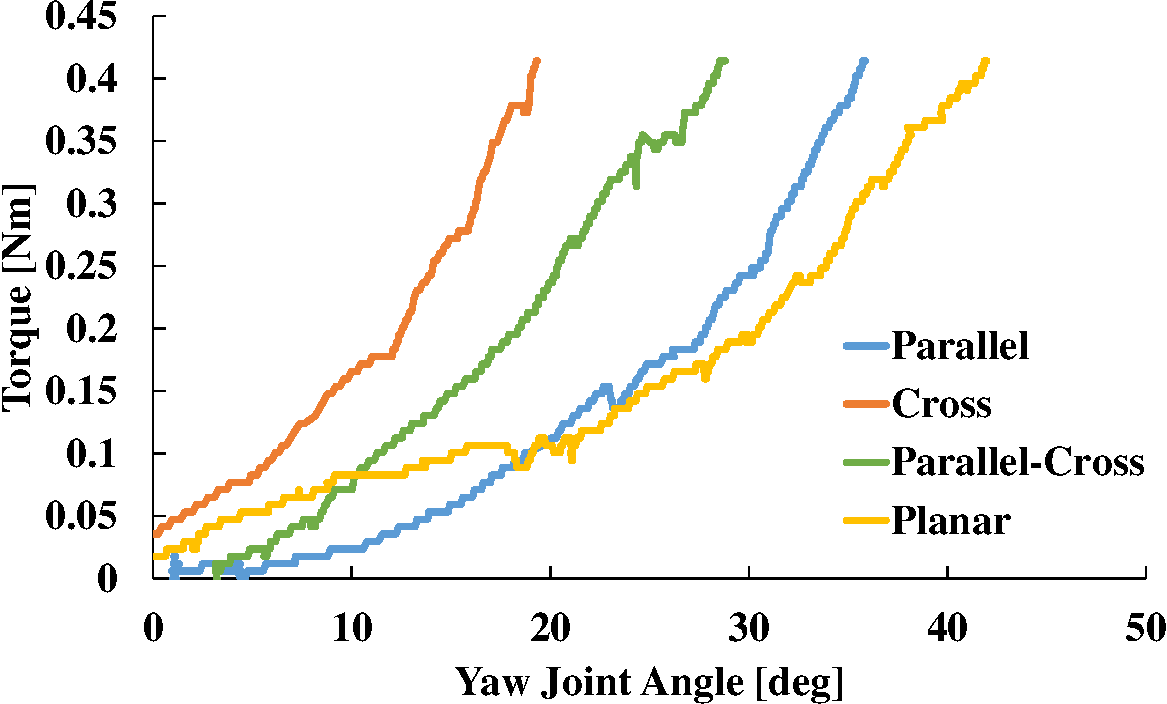
\includegraphics[width=0.9\columnwidth]{figs/passive-compliance.pdf}
  \vspace*{-4mm}
  \caption{Passive compliance by collateral ligaments}
  \label{fig:passive-compliance}
\end{figure}

\subsection{膝関節への適用-終末強制回旋機能}
面状牽引構造による靭帯によって膝関節の終末強制回旋機能を再現することで、人体のような複雑な可動域が実現されることを確認する。終末強制回旋機能とは、膝屈曲状態で回旋自由度を許して複雑な動作を可能にする一方、筋のモーメントアームが小さくなる膝伸展姿勢では靭帯と骨格形状、そして大腿四頭筋によって回旋角度を正面に収束させロックして関節を安定化させる機能である。筋骨格ヒューマノイドではリジッドな機構で実現した研究\cite{IROS2013:asano:knee}がなされているが、膝伸展時に衝撃がかかることによって軸が折れるなど致命的な破壊が起きうる。複雑な可動域の実現だけでなく人体のように腱や靭帯による衝撃吸収可能なソフトな拘束が重要であり、前節で実装した布による面状牽引構造によってその両立が可能となる。

\reffig{fig:ovv-knee}に側副靭帯と筋を取り付けた膝関節の概要を示す。大腿四頭筋筋として用いたモータは90Wと120Wが一本ずつで両者とも減速比は53:1である。擬似球関節の一本の回転軸を固定し、回旋と屈曲(\reffig{fig:ovv-knee}のYawとPitch)方向の回転を許す。
終末強制回旋機能は大腿四頭筋によっても起きるため本来ワイヤは下腿の骨格に取り付けるべきだが、靭帯による影響のみを検証するため大腿の筋が回旋トルクを生じさせないように取り付けた。
膝を屈曲させた状態で回旋させ、モータによってワイヤに20Nの張力をかけ膝を伸展させたところ、側副靭帯による関節受動トルクによって終末強制回旋機能が生じることが確認された(\reffig{fig:shm})。膝関節の伸展に応じて正面方向へ関節がロックされている。
膝屈曲状態で回旋角度を適当にとり、10回にわたって膝を伸展させた際の膝の回旋角度の様子を\reffig{fig:shm-graph}に示す。複数の姿勢から膝の伸展に応じて回旋が生じ、関節角度が収束していることが分かる。

\begin{figure}[tb]
 \centering
  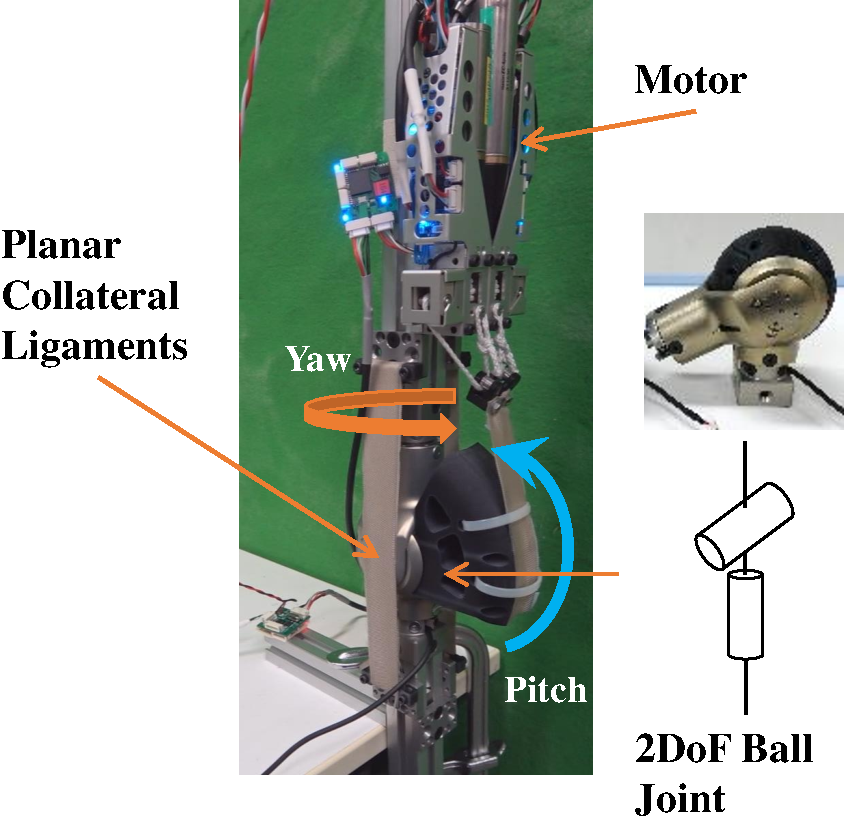
\includegraphics[width=1.0\columnwidth]{figs/ovv-of-robot.pdf}
  \vspace*{-4mm}
  \caption{Overview of the knee joint with planar collateral ligaments and muscle unit.}
  \label{fig:ovv-knee}
\end{figure}

%% \begin{figure}[tb]
%%  \centering
%%   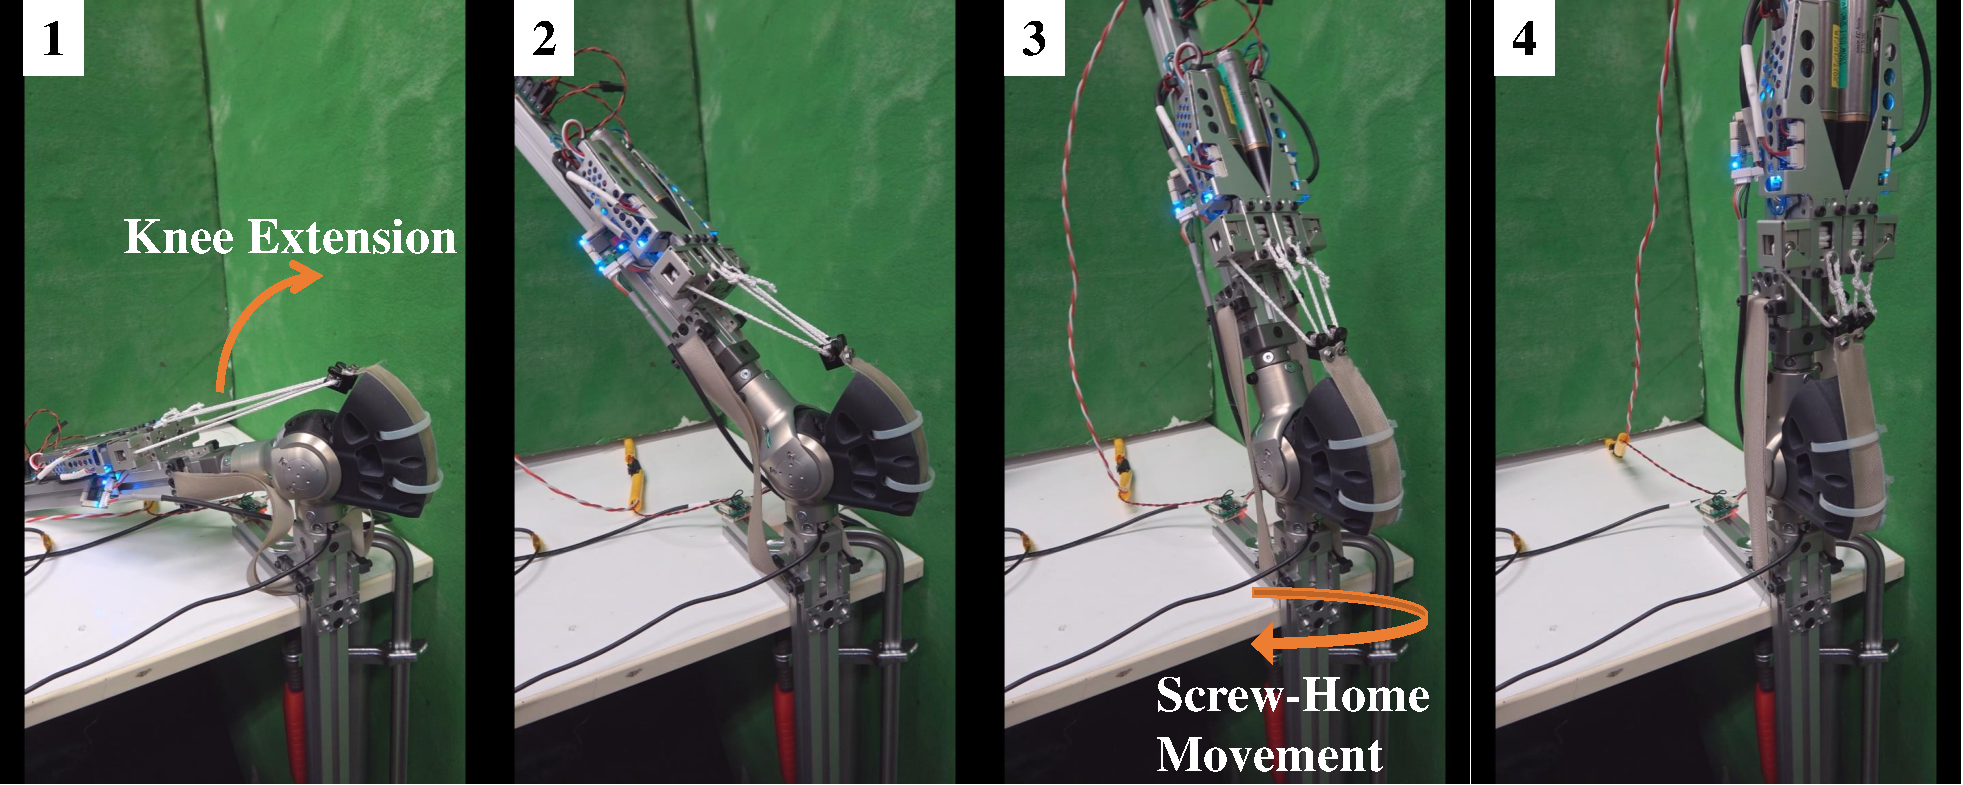
\includegraphics[width=1.0\columnwidth]{figs/screw-home.pdf}
%%   \vspace*{-4mm}
%%   \caption{Screw-home movement of the knee joint which yaw angle is converged by its collateral ligaments as pitch angle extends.}
%%   \label{fig:shm}
%% \end{figure}

\begin{figure*}[tb]
 \centering
  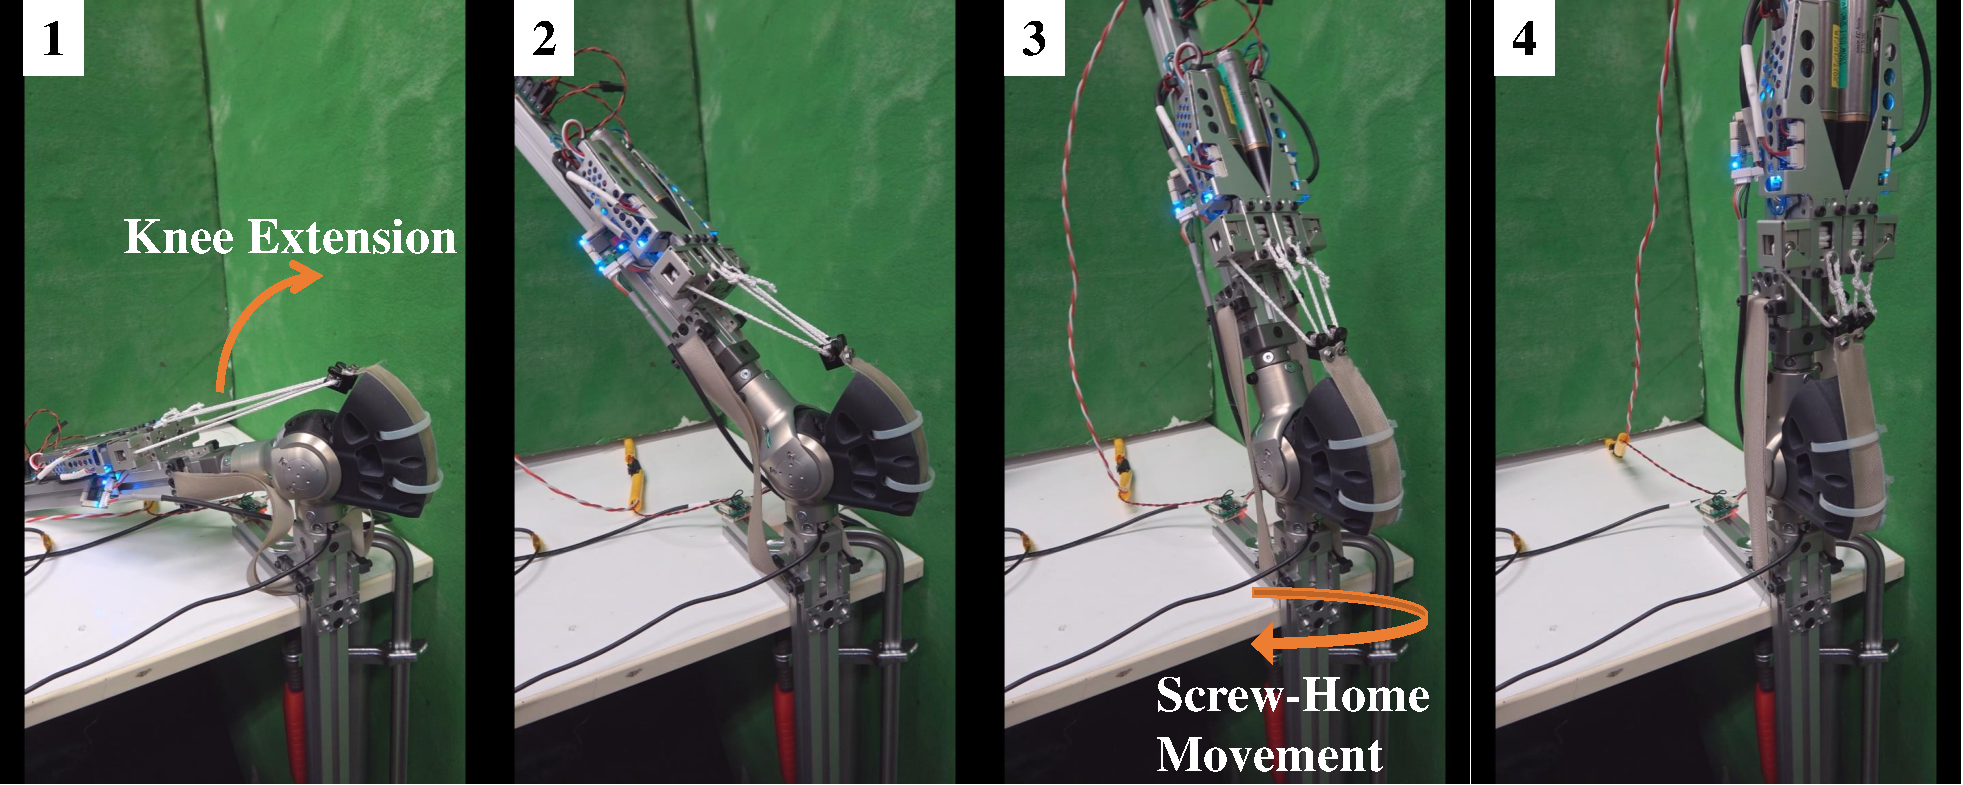
\includegraphics[width=1.0\textwidth]{figs/screw-home.pdf}
  \vspace*{-4mm}
  \caption{Screw-Home movement of knee joint which angle is converged by collateral ligaments.}
  \label{fig:shm}
\end{figure*}

\begin{figure}[tb]
 \centering
  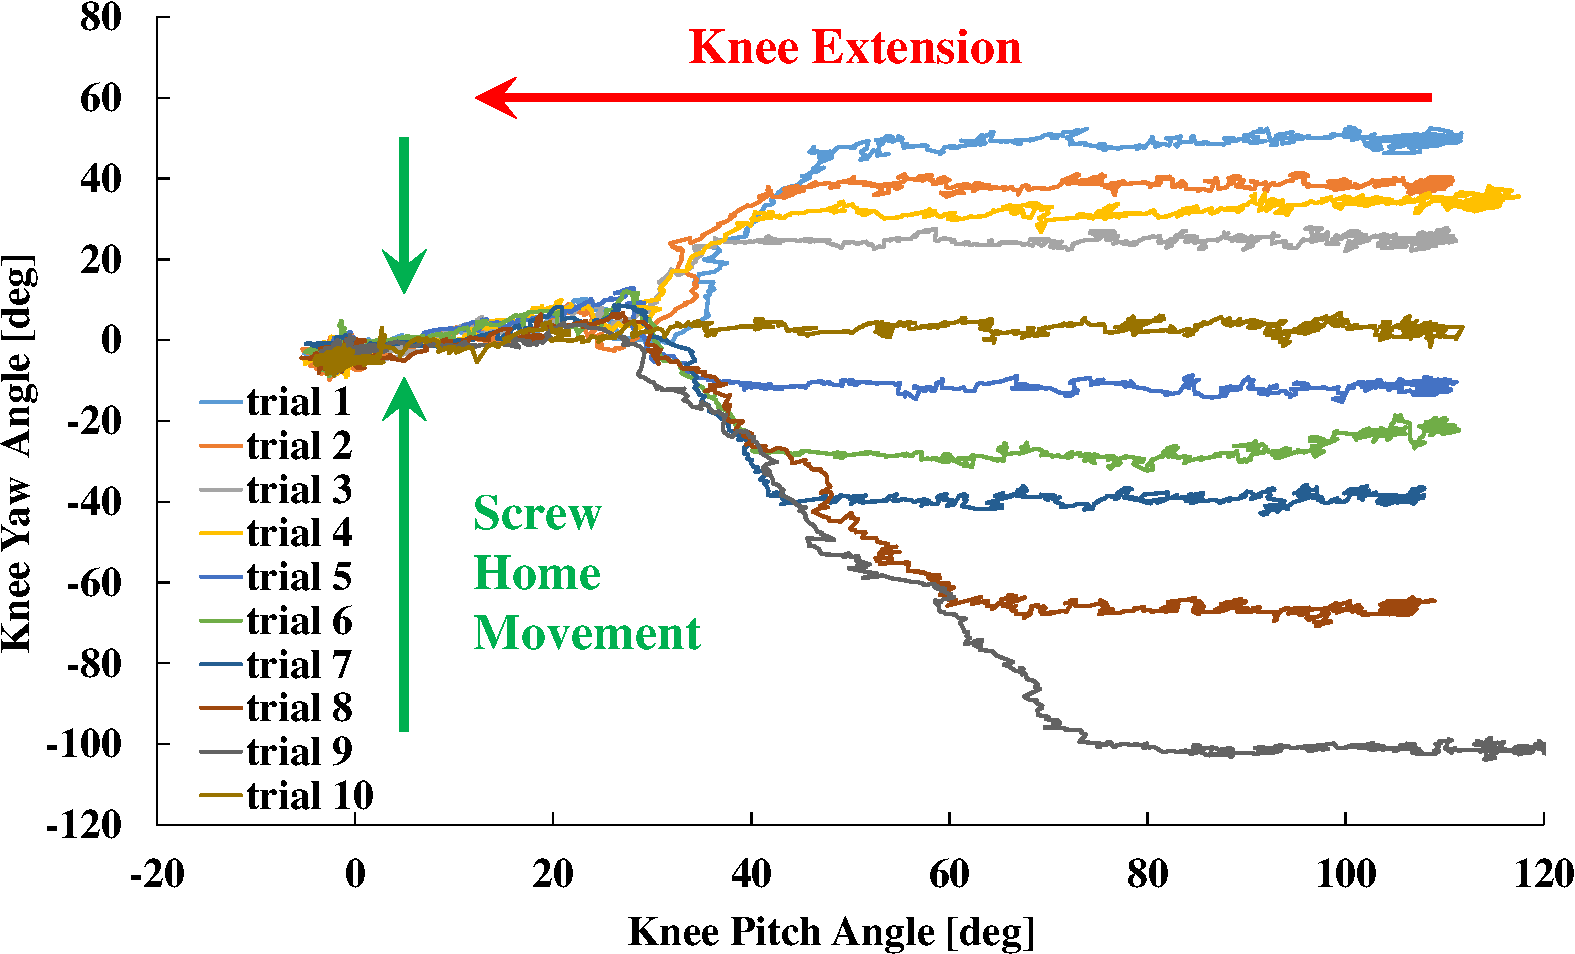
\includegraphics[width=1.0\columnwidth]{figs/screw-home-convergence.pdf}
  \vspace*{-4mm}
  \caption{Relation between pitch angle and yaw angle of the knee joint during screw-home movement.}
  \label{fig:shm-graph}
\end{figure}

\section{結論}
筋骨格ヒューマノイドにおいて、関節をまたいで骨格間を牽引する筋や靭帯が、関節の姿勢の変化などによって意図しない経路をとらず安定して張力を発揮することが重要である。本研究では筋骨格ヒューマノイドの骨格間を牽引する構造として、これまでのワイヤによる線状牽引構造に対する面状牽引構造の利点を示し、張力に対する性質を評価した。次に従来のリジッドな関節可動域拘束に対し、柔軟な面状牽引構造を有する靭帯によって人体のような複雑な可動域の実現が可能であることを示した。柔らかい靭帯による衝撃吸収による破損の回避や、動的動作を行った際に筋と共に弾性エネルギーを蓄えることができると期待される。

靭帯は骨格形状と共に関節の運動方向を決定する役割を持ち、人体の開放型関節では並進方向の運動の拘束も担う。今回用いた擬似球関節では、機構によって並進方向の自由度は既に拘束され、靭帯は回転方向のみの拘束をしている。このため回転軸に対するせん断方向の力は柔軟構造によって吸収することは出来ない。開放型関節は軸ではなく骨格の面で力を受けるので、軸で力を受ける機構より壊れづらいと考えられる。靭帯の開放型関節への適用は今後の課題となる

人体には面状の構造が多数存在する。大殿筋はその好例で、股関節を覆うことで様々な関節姿勢でトルクを発揮することができる。今後の展望として、腸骨大腿靭帯などの柔軟な可動域制限を有し、面状牽引構造を持った筋によって安定した股関節トルクが発揮可能な骨盤の開発をしていきたい。

\section{謝辞}
本研究の一部はトヨタ自動車株式会社の支援を受けて行われた。

\footnotesize
\bibliographystyle{robomech}
\bibliography{main}

\normalsize
\end{document}
